\subsection{Amortecimento das oscilações betatron}\label{sec:4.3}
Já é hora de analisar o amortecimento por radiação das oscilações betatron. Aqui será dado apenas um tratamento aproximado, porém por meio de um método que -- com apenas um pouco de álgebra -- pode ser estendido a um cálculo exato. De qualquer forma, o resultado exato é mais facilmente obtido por um teorema geral que será discutido na \autoref{sec:4.4}.

Começando pelas oscilações betatron verticais (a notação será a mesma usada na \autoref{part2}). O movimento será aproximado ignorando a variação de $\beta$ com $s$, então pode-se escrever (veja a \autoref{sec:2.8}):
\begin{align}
	z = A\ cos(\varphi), \ \ z' = \frac{A}{\beta}\ sen(\varphi)\label{eq:4.24}
\end{align}
onde $\varphi = s/\beta$. A amplitude de oscilação $A$ pode ser obtida por $z$ e $z'$ em qualquer instante por
\begin{align}
	A^2 = z^2 + (\beta z')^2
\end{align}
Suponha um elétron com energia nominal $E_0$ -- o qual está oscilando verticalmente sobre a órbita ideal. Em qualquer elemento azimutal $\delta s$ o elétron irá perder por radiação uma pequena quantidade de energia $\delta E$. Seu vetor de momento $p$ será mudado por $\delta p$ e, como foi apontado anteriormente, $\delta p$ é paralelo (e oposto) a $p$, então $|\delta p| = \delta E/c$. Veja a \autoref{fig:fig40}(a). A perda por radiação não muda nem o desvio nem a inclinação da trajetória (as variações de $z$ e de $s$ com relação ao tempo existem, mas compensam uma a outra); então a amplitude $A$ não é alterada pela radiação. Existe um pequeno efeito causado pelas forças focalizadoras efetivas e, portanto, $\beta$ também varia com uma mudança na energia. Este efeito é chamado de amortecimento adiabático, porém é um efeito de segunda ordem e pode ser ignorado nesta análise já que a energia não varia na média quando a aceleração de RF é considerada.

\begin{figure}[!htb]
	\centering
	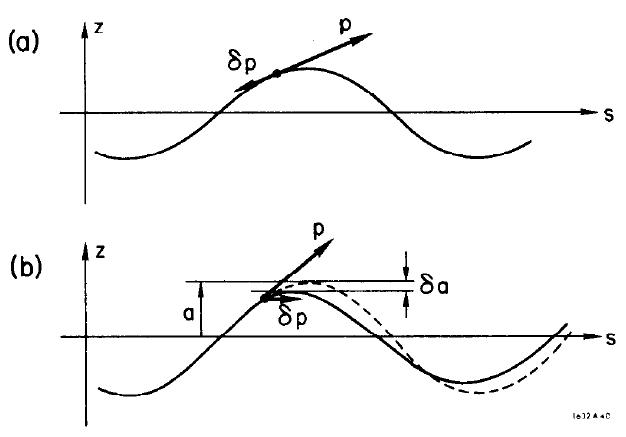
\includegraphics[width=0.7\linewidth]{./Figuras/fig40.jpeg}
	\caption{Efeito da mudança de energia nas oscilações betatron verticais: (a) por perda por radiação, (b) por aceleração de RF. Retirado de \cite{sands1970physics}.}
	\label{fig:fig40}
\end{figure}

Agora, note que o efeito da força de aceleração de RF é um pouco diferente. Esta força é, na média, paralela à órbita ideal. Então o incremento de momento $\delta p$ recebido no elemento azimutal $\delta s$ não é mais exatamente paralelo a $p$. Veja a \autoref{fig:fig40}(b). Seja $p_\perp$ a componente  de $p$ perpendicular à órbita ideal; então, como os ângulos são pequenos, pode-se aproximar
\begin{align*}
	z' = \frac{p_\perp}{p}
\end{align*}
Novamente, a força de aceleração não muda $z$. Mas, de fato, muda $z'$ que, considerando apenas termos lineares, vai para
\begin{align}
	z' \rightarrow \frac{p_\perp}{p+\delta p} = \frac{p_\perp}{p}\left(1-\frac{\delta p}{p}\right) = z'\left(1-\frac{\delta p}{p}\right)
\end{align}
Assim, mudança em $z'$ é
\begin{align}
	\delta z' = -z'\frac{\delta p}{p} = -z'\frac{\delta E}{E}
\end{align}
Existe uma mudança correspondente na amplitude $A$;
\begin{align}
	A\delta A = \beta^2 z' \delta z' = -(\beta z')^2 \frac{\delta E}{E}
\end{align}

\begin{proof}
	Considerando que o movimento vertical é dado pela equação \eqref{eq:4.24}, então, considerando variações $z'$ e $A$, tem-se que
	\begin{align*}
		z = (A+\delta A)\ cos(\varphi), \ \ (z' + \delta z') = \frac{(A+\delta A)}{\beta}\ sen(\varphi)
	\end{align*}
	Logo, por relação trigonométrica, obtém-se que
	\begin{align*}
		(A+\delta A)^2 &= z^2 + (\beta (z'+\delta z'))^2\\
		A^2+2 A \delta A + \delta A^2 &= z^2 + \beta^2 (z'^2 + 2z'\delta z' + \delta z'^2)
	\end{align*}
	Descartando os temos de segunda ordem:
	\begin{align*}
		2 A \delta A &= \beta^2 2z'\delta z'\\
		\therefore A\delta A &= \beta^2 z' \delta z'
	\end{align*}
	c.q.d.
\end{proof}

Agora, a fase de oscilação na chegada do elétron no ponto $s$ é arbitrária (e todos os valores entre $0$ e $2\pi$ são igualmente prováveis) então apenas a mudança média em $A$ importa. A média de $(z'^2)$ é $A^2/2\beta^2$, então
\begin{align}
	A\mean{\delta A} = -\frac{A^2}{2}\frac{\delta E}{E_0}
\end{align}

Suponha que todos os elementos do ganho de aceleração sejam somados em uma revolução. Como a soma de todos os $\delta E$ deve resultar em $U_0$, obtém-se que a mudança $\Delta A$ que ocorre em $A$ em uma revolução (devido à aceleração de RF) é
\begin{align}
	\frac{\Delta A}{A} = -\frac{U_0}{2E_0}\label{eq:4.30}
\end{align}
Como $\Delta A$ em cada período de revolução $T_0$ é proporcional a $A$, o movimento é amortecido exponencialmente -- como $e^{-\alpha_z t}$. Ou seja,
\begin{align}
	\frac{1}{A}\frac{dA}{dt} = \frac{\Delta A}{A T_0} = -\frac{U_0}{2E_0T_0}
\end{align}
então o coeficiente de amortecimento é
\begin{align}
	\alpha_z = \frac{U_0}{2E_0T_0} = \frac{\mean{P_\gamma}}{2E_0}
\end{align}
Pode-se mostrar que um cálculo exato -- usando a forma completa das oscilações betatron verticais -- leva ao mesmo resultado. Note que a taxa de amortecimento das oscilações verticais é apenas $1/2$ da taxa típica das oscilações de energia (quando $\mathscr{D}$ é pequeno); veja a equação \eqref{eq:4.20}.

É muito importante notar que o amortecimento "por radiação" não ocorre no processo de perda por radiação, mas sim no processo de ganho de energia do sistema de RF. Isto poderia ser um motivo de questionamento sobre o nome "amortecimento por radiação". Mas, pensando bem, não existiria oportunidade para amortecimento pelos campos de RF se não fosse necessário compensar a perda de energia por radiação. Então o nome "amortecimento por radiação" não é tão ruim.

Agora, hora de analisar os efeitos da radiação sobre as oscilações betatron radiais. Num primeiro momento, pode-se pensar que as oscilações betatron radiais deveriam ser amortecidas do mesmo modo que as verticais. Porém existem complicações adicionais que fazem com que este problema deva ser tratado separadamente. Um novo elemento aparece devido à mudança do deslocamento betatron que ocorre quando existe uma mudança na energia. Lembre-se que o deslocamento radial total $x$ é a soma de duas partes: o deslocamento $x_\epsilon$ da órbita fechada e o deslocamento beatron $x_\beta$ com relação a esta órbita,
\begin{align}
	x = x_\epsilon + x_\beta\label{eq:4.33}
\end{align}

Quando a energia de um elétron muda por uma quantidade $\delta E$, existe uma mudança em $x_\epsilon$ pela quantidade, veja a equação \eqref{eq:2.28},
\begin{align}
	\delta x_\epsilon = \eta \frac{\delta E}{E_0}
\end{align}
Mas, como a posição do elétron no espaço não muda por um impulso momentâneo finito, o deslocamento total $x$ não muda, então obrigatoriamente existe uma compensação em $x_\beta$. Isto é, da equação \eqref{eq:4.33},
\begin{align*}
	\delta x = \delta x_\epsilon + \delta x_\beta = 0
\end{align*}
de forma que
\begin{align}
	\delta x_\beta = -\delta x_\epsilon = -\eta \frac{\delta E}{E_0}\label{eq:4.35}
\end{align}
Quando ocorre uma variação na energia, o elétron não se move instantaneamente, mas o eixo de referência das suas oscilações sim e o deslocamento com respeito a este eixo é, portanto, alterado --  como é ilustrado na \autoref{fig:fig41}.

\begin{figure}[!htb]
	\centering
	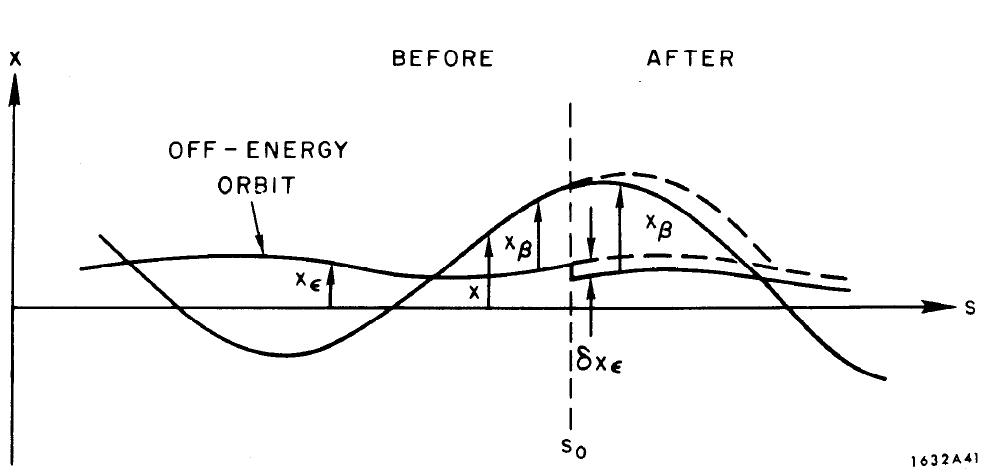
\includegraphics[width=0.9\linewidth]{./Figuras/fig41.jpeg}
	\caption{Efeito de uma mudança repentina de energia em $s_0$ sobre o deslocamento betatron radial. Retirado de \cite{sands1970physics}.}
	\label{fig:fig41}
\end{figure}

Algo similar ocorre na inclinação betatron. Correspondendo à equação \eqref{eq:4.33}, tem-se
\begin{align}
	x' = x'_\epsilon + x'_\beta
\end{align}

Agora, porém, um impulso elementar pode mudar a inclinação total $x'$ por algum $\delta x'$, então deve-se ter
\begin{align}
	\delta x'_\beta = \delta x' - \delta x'_\epsilon
\end{align}
Tomando a derivada de $x_\epsilon$ da equação \eqref{eq:2.28},
\begin{align}
	\delta x'_\beta = \delta x' - \eta' \frac{\delta E}{E_0}\label{eq:4.38}
\end{align}
onde $\eta'$ é, claro, $d\eta/ds$. Mesmo que $\delta x'$ seja zero, uma mudança na inclinação de $x_\epsilon$ -- o eixo de referência da oscilação -- produziria uma mudança na inclinação da oscilação betatron.

Existe mais uma complicação adicional devido à curvatura da órbita de referência. As metades positiva e negativa de uma oscilação betatron ocorrem em intervalos iguais de $s$, mas o elétron viaja um comprimento de caminho maior na parte positiva do que na negativa --  veja a equação \eqref{eq:3.7}. Apesar do efeito total sobre o comprimento de caminho ser nulo em uma revolução completa, existe, em geral, uma diferença na quantidade de energia perdida por radiação durante as duas metades da oscilação. E a amplitude da oscilação é, logo, afetada.

Aplicando, agora, estas ideias sobre a perda por radiação $\delta E$ em um elemento azimutal $\delta s$. Um cálculo preciso pode ser feito a partir das mudanças em $x$ e $x'$ obtidas nas equações \eqref{eq:4.35} e \eqref{eq:4.38}. Porém, mantendo as aproximações feitas anteriormente, pode-se fazer uma suposição simplificada de que $\eta$ é uma constante, então $\eta'=0$; e escrever a variação de $x_\beta$ com $s$ na mesma forma que a variação betatron vertical, ou seja,
\begin{align}
	x_\beta = A\ cos(\varphi), \ \ x'_\beta = \frac{A}{\beta}\ sen(\varphi)
\end{align}
Desta vez, tem-se que
\begin{align}
	A \delta A = x_\beta \delta x_\beta + \beta^2 x'_\beta \delta x'_\beta
\end{align}
Pela suposição de que $\eta$ é constante, $x'_\epsilon = 0$. Logo, $x' = x'_\beta$ e $\delta x' = \delta x'_\beta$, então uma mudança de energia não causa variação na inclinação. Logo, $\delta x_\beta = 0$ e
\begin{align}
	A \delta A = -x_\beta \eta \frac{\delta E}{E_0}\label{eq:4.41}
\end{align}

Novamente, toma-se o desvio de energia $\delta E$ como a perda por radiação em um elemento azimutal $\delta s$. Para o movimento vertical, assumiu-se que o elétron estava sempre se movendo com deslocamento radial nulo, então a taxa de perda por radiação era a mesma (até termos de primeira ordem em $x$) que a taxa de perda de energia na órbita ideal. Já para o movimento radial, se os ímãs possuem gradiente de campo, as coisas são um pouco diferentes. Para simplificar a discussão, a análise será sobre um campo guia isomagnético de função separável. Em uma máquina com função separável, a taxa de perda por radiação independe de $x$ -- até termos de primeira ordem.\footnote{Há apenas gradiente de campo nos quadrupolos; onde $B$ é proporcional a $x$. Como a taxa de radiação varia com $B^2$, não há efeito de primeira ordem.}Desta forma, pode-se considerar que, para um elétron com energia nominal, a taxa de perda por radiação $P_\gamma(s)$ não depende de $x$, apenas de $s$. Então, a variação de energia em um elemento de caminho $\Delta \ell$ é
\begin{align}
	\delta E = -\frac{P_\gamma}{c}\Delta \ell
\end{align}

Tomando $\Delta \ell$ da expressão em \eqref{eq:2.15},
\begin{align}
	\delta E = -\left(1+\frac{x_\beta}{\rho_s}\right)\frac{P_\gamma}{c}\Delta s
\end{align}

Combinando este resultado com a equação \eqref{eq:4.41}, tem-se que a mudança de amplitude é
\begin{align}
	A \delta A = x_\beta \eta \left(1+\frac{x_\beta}{\rho_s}\right)\frac{P_\gamma}{cE_0}\Delta s
\end{align}
Novamente, apenas o valor esperado de $\delta A$ é importante -- a média sobre todos os ângulos de fase $\varphi$. O valor esperado de $x_\beta$ é zero e de $x_\beta^2$ é $A^2/2$; então tem-se que
\begin{align}
	\frac{\mean{\delta A}}{A} = \frac{\eta}{2 \rho_s}\frac{P_\gamma}{cE_0}\Delta s
\end{align}

Como foi assumido um campo guia isomagnético, em qualquer lugar que $P_\gamma$ for diferente de 0, $\rho = \rho_s = 1/G_0$ e pode-se somar o efeito em cada $\Delta s$ para obter a variação $\Delta A$ em uma revolução completa. A soma de todos os termos $P_\gamma s/c$ é apenas a perda de energia $U_0$ em uma volta completa. Então o efeito da radiação é
\begin{align}
	\left(\frac{\Delta A}{A}\right)_{rad} = \frac{\eta}{2 \rho_0}\frac{U_0}{E_0}
\end{align}
Observe que o sinal do lado direito da equação é positivo. Ou seja, há um aumento da amplitude devido à radiação!

Felizmente, esta é apenas uma parte da análise. Também é preciso considerar o efeito da aceleração de RF. Porém, existe um efeito de "tamanho de caminho" correspondente. Geralmente, as cavidades de RF são localizadas onde $\rho = \infty$, ou seja, em trechos retos. Mas, de qualquer forma, é uma propriedade destas cavidades que o ganho de energia seja (até primeira ordem, ao menos) independente do deslocamento betatron. O cálculo da contribuição da aceleração de RF ocorre da mesma forma que no movimento vertical, com o resultado da equação \eqref{eq:4.30}. Para obter o efeito total em uma revolução é preciso computar as contribuições da perda por radiação e da aceleração para obter
\begin{align}
	\frac{\Delta A}{A} = -\left(1-\frac{\eta}{\rho_0}\right)\frac{U_0}{2E_0}
\end{align}
o que gera o coeficiente de amortecimento $\alpha_x$ das oscilações radiais
\begin{align}
	\alpha_x = \left(1-\frac{\eta}{\rho_0}\right)\frac{U_0}{2E_0T_0}\label{eq:4.48}
\end{align}
Um cálculo preciso para um campo guia isomagnético de função separável chega neste mesmo resultado se $\eta$ por substituído por $\mean{\eta}_{mag}$, o valor médio de $\eta(s)$ no ímãs. Mas retomando a equação \eqref{eq:3.14}, $\mean{\eta}_{mag} = \alpha R$ então
\begin{align}
	\alpha_x = \left(1-\frac{\alpha R}{\rho_0}\right)\frac{U_0}{2E_0T_0}\ \ (isomag.\ e\ fun. sep.)\label{eq:4.49}
\end{align}

Considerando que $\alpha R/\rho_0$ é menor que 1 -- como este termo usualmente é -- o coeficiente de amortecimento é positivo e as oscilações radiais são amortecidas. Mas existe um efeito "anti-amortecimento" da radiação -- o termo $\alpha R/\rho_0$ -- que vai contra o amortecimento positivo do sistema. Enquanto o termo anti-amortecimento for pequeno, este não causa problema algum.

Comparando a equação \eqref{eq:3.49} com os resultados da \autoref{sec:4.2} é possível observar que o resultado também pode ser escrito em termos de $\mathscr{D}$\footnote{Este resultado é obtido mudando um pouco as aproximações feitas: ao invés de considerar que há um $\delta x'$ e considerar $\eta$ constante, considere que $\delta x'=0$ e considere a variação de $\eta$ com $s$.}:
\begin{align}
	\alpha_x = (1-\mathscr{D})\frac{U_0}{2E_0T_0}\ \ (geral)\label{eq:4.50}
\end{align}
Apesar deste resultado ter sido obtido apenas para um tipo específico de campo guia (e com algumas aproximações), a equação \eqref{eq:4.50} é exata para qualquer campo guia. Isto é, se a variação de $\eta$ com $s$ tivesse sido considerada, no lugar do termo $\eta/\rho_0$ na equação \eqref{eq:4.48} haveria a expressão completa de $\mathscr{D}$ da equação \eqref{eq:4.17}. Mais será dito a seguir sobre esta interessante "coincidência".